\documentclass[11pt]{article} % do not change this line
\input{BigDataStyle.txt}      % do not change this line
\usepackage{amsmath,amsfonts,amssymb,amsthm,latexsym,graphicx}
\usepackage{url}

\emergencystretch=5mm
\tolerance=400
\allowdisplaybreaks[4]

\graphicspath{ {./images/} }

\theoremstyle{plain}
\newtheorem{theorem}{Theorem}[section]
\newtheorem{proposition}[theorem]{Proposition}
\newtheorem{corollary}[theorem]{Corollary}
\newtheorem{lemma}[theorem]{Lemma}
\newtheorem{problem}[theorem]{Problem}

\theoremstyle{definition}
\newtheorem*{remark}{Remark}

\title{Deep Learning}
\author{Michael Harrison}

\newcommand{\Programme}{Machine Learning}
% Computational Finance students: uncomment the next line
%\twodepartmentstrue

\begin{document}
\maketitle

\declaration

\begin{acknowledgement}
I would like to thank...
\end{acknowledgement}

% NB: The abstract environment also inserts the Table of Contents
\begin{abstract}
ABSTRACT TBD
\end{abstract}


% BEGIN INTRODUCTION
\newpage
\setcounter{page}{1}
\pagenumbering{arabic}
\section{Introduction}
The aim of this project is to explore the use of Deep Learning in a practical situation. Deep Learning techniques have been used in a range of problems, such as image recognition [ref GoogleLeNet], natural language processing [ref Google Neural Machine Translation], playing games [ref AlphaGo] and self-driving cars [ref WayMo], among others. These techniques have often achieved cutting-edge performance on these tasks - for instance, surpassing human performance in the ImageNet task [ref ILSVRC], or beating the world champion Lee Sedol at the game Go [ref AlphaGo win]. As such, Deep Learning is an exciting branch of Machine Learning with the potential to make significant impacts in many areas of life. Indeed Deep Learning is one of (the?) largest areas of active research in Machine Learning at the time of writing [ref numbers of citations].
\\
\\
\noindent
This project focuses on image recognition, as this is one of the areas where Deep Learning has seen its biggest successes. In particular, we will be applying Deep Learning to the MURA (\textbf{mu}sculoskeletal \textbf{ra}diographs) dataset, published by the Machine Learning Group at Stanford University \cite{MURA2017}. This is a collection of 40,005 X-ray images of a part of the upper extremity - comprising the arm, shoulder, wrist, hand etc. Each image is from one of 14,656 studies of an individual patient, performed at a particular point in time on one of these parts of the upper extremity. Each study was labelled as normal or abnormal at the time of clinical interpretation by a radiologist from Stanford Hospital - and these labels have been published alongside the images themselves. Therefore the aim of this project is to use Deep Learning to perform binary image classification on this set of X-rays - classifying them as either normal or abnormal. This will be a supervised learning task, since we have clear labels for our data, and our aim is to predict them. 
\\
\\
\noindent
While any model developed as part of this project can only represent a toy solution to this problem, the principle of combining Deep Learning and medicine seems to be a good one. Inded this too is an area of active research, both within radiology [ref radiology], medical imaging [ref other DL/med image work] and medicine more widely [ref DL/med work]. The works cited of course represents only a small fraction of what is being done. Thinking optimistically, Deep Learning can help improve patient outcomes, produce results more quickly, alleviate pressure off medical pracitioners, reduce medical mistakes and improve medical decision-making. As such, this represents good motivation for me to dip my toe into this area as part of my project.

% END INTRODUCTION


% BEGIN BACKGROUND
\newpage
\section{Background}
This section describes the background of Deep Learning, and the methodology behind the techniques used in this project.

\subsection{Deep Learning}
The main idea behind Deep Learning is for a system to learn representations of the data given to it. While these representations can start out simple, they are organised into a hierarchical sequence of layers so that simpler representations from earlier layers can be composed and built up into higher-level, more complex representations. This is repeated over many layers so that the final representations have sufficient information and detail for the task at hand. This process of building up complex representations from simpler parts means that feature engineering - the choice of which aspects of the data to include in the model, how they should be transformed or combined etc - is performed automatically by the system, as part of training. This is one of the great strengths of Deep Learning since feature engineering as a manual process can be difficult and time-consuming, especially when the data is very high-dimensional (as with images).       

\subsection{Artificial Neural Networks}
\subsubsection{Basic Structure}
More specifically, these Deep Learning systems tend to be artificial neural networks (ANN's), of various forms depending on the nature of the task. A simple version of such a network \cite{wiki:simple_ann} is shown in \textbf{Figure \ref{fig:simple_ann}} below. These consist of a set of "neurons" (the circles in the image below) organised into layers, with each neuron from one layer connected to all neurons in the next layer. Each neuron has an associated activation, typically just a real number, which is derived from the activations of the neurons feeding into it from the previous layer. The input layer is a special case, where the neuron activations represent values from the item of data being fed into the network. For instance, for greyscale images, the input neurons correspond to each pixel in the given input image, and the input activations are simply each pixel's value. The activations of the final output layer may represent different things, depending on the task - for instance, the final learned representation of the data item when doing dimension reduction. Or, for classification, the probability distribution over the set of classes that captures the network's prediction of which class the given data item is in. 
\begin{figure}[!ht]
  \centering    
  \caption{Example of a simple artificial neural network}
  \label{fig:simple_ann}
  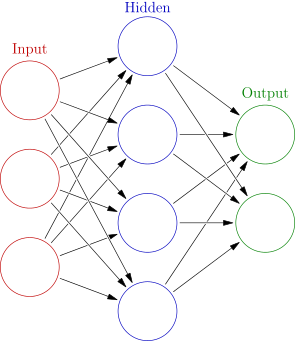
\includegraphics[scale=0.5]{simple_ann.png}
\end{figure}
\\
\\
\noindent
The connections between the neurons from one layer to the next represent the network's weights, each weight again usually just a real number. In addition to these weights between layers, each neuron (aside from the input layer) has an associated bias, once again usually just a real number. Taken across the whole network, these weights and biases form the set of parameters that define the model. They dictate how the activations from neurons in the previous layer should be used to calculate the activations of neurons in the next layer. For instance, let the activations of the neurons in layer \(i\) be given by the vector \(a_i\), and the weights connecting neurons in layer \(i\) to those in layer \(i+1\) be given by the matrix \(\mathbf{W_{i+1}}\). So if the numbers of neurons in layers \(i\) and \(i+1\) respectively are \(n_i\) and \(n_{i+1}\), then \(a_i\) will have dimension \((n_i,1)\), and \(\mathbf{W_{i+1}}\) dimension \((n_i,n_{i+1})\)\footnote{Each of the \(n_i\) neurons in layer \(i\) connects to each of the \(n_{i+1}\) neurons in layer \(i+1\), making \({n_i}\times{n_{i+1}}\) connections in total.}. Then the activations for the neurons in layer \(i+1\) are given by:
\[a_{i+1} = f_{i+1}(\mathbf{W_{i+1}^{\top}}a_i + b_{i+1}) \]
where:
\begin{itemize}
  \item \(b_{i+1}\) is the vector of biases for the neurons in layer \(i+1\) (so of dimension \((n_{i+1},1)\)). 
  \item \(f_{i+1}\) is the activation function for layer \(i+1\), that applies element-wise to the vector on which it operates, and hence returns a vector. The choice of activation functions is part of the design of the network.   
\end{itemize}
This process is repeated, with activations from the input layer feeding into activations of the first hidden layer; activations from this hidden layer feeding into the next hidden layer; etc until the final activations in the output layer are produced. Note that while \textbf{Figure \ref{fig:simple_ann}} above showed only one hidden layer between input and output, in practice there can be arbitrarily many hidden layers - each taking as input the activations from their previous layer, and sending their own activations as output to the next layer. The choice of the numbers of hidden layers, and the numbers of neurons in each of these layers is again part of the design of the network.   

\subsubsection{Activation Functions}
The activation functions are usually chosen to be non-linear - since otherwise, composing several layers of neuron activations reduces to taking a linear function of the original input neurons and the network itself simply becomes a linear function. To see this, let \(f(x) = x\) be the linear activation function used throughout the network. Then if layer \(0\) is the input layer, the activations of layer \(1\) are:
\[a_{1} = f(\mathbf{W_1^{\top}}a_0 + b_1) = \mathbf{W_1^{\top}}a_0 + b_1\]
And hence the activations for layer \(2\) are:
\begin{align}
a_{2} &= f(\mathbf{W_2^{\top}}a_1 + b_2)  \\
      &= \mathbf{W_2^{\top}}a_1 + b_2 \\
      &= \mathbf{W_2^{\top}}(\mathbf{W_1^{\top}}a_0 + b_1) + b_2 \\
      &= \mathbf{(W_1W_2)^{\top}}a_0 + \mathbf{W_2^{\top}}b_1 + b_2 \\
      &= \mathbf{W'^{\top}}a_0 + b' 
\end{align}
where:
\begin{itemize}
  \item \(\mathbf{W'} = \mathbf{W_1W_2}\)  is an \({n_0}\times{n_2}\) matrix
  \item \(b' = \mathbf{W_2^{\top}}b_1 + b_2\) is an \({n_2}\times{1}\) vector
  \item Equation \((4)\) uses the matrix transpose rule \((AB)^{\top} = B^{\top}A^{\top}\)
\end{itemize}
Hence both \(a_1\) and \(a_2\) are linear functions of \(a_0\). This argument can be extended to any number of hidden layers, and so the output of the whole network (regardless of its size) is simply a linear function of the input. This is undesirable since such a network cannot learn more complicated, non-linear features of the data. Training the network is effectively equivalent to just performing linear regression.
\\
\\
\noindent
Therefore non-linear activation functions are usually preferred. In this project we have used the following activation functions, in line with standard practice for image classification [ref e.g. VGG16].
\\
\\
\noindent
\textbf{ReLU}
\\
\noindent
The Rectified Linear Unit (ReLU) is a scalar activation function that takes a linear function of its argument above a certain threshold \(m\), and is constant otherwise:
\[f(x) = max\{x,m\} \] 
Note that \(m\) is a hyperparameter, specified in advance of training, rather than learning during it. Typically it is just set to 0 - as otherwise this implies some sort of prior knowledge about the scale of the "pre-activation" values \(\mathbf{W_{i+1}^{\top}}a_i + b_{i+1} \) for all the various layers and neurons in the network (since \(m\) could theoretically be set on a neuron-by-neuron basis). This would be difficult to justify, especially when adjusting the level of these pre-activation values is already handled by the bias term \(b_{i+1}\), a parameter that is learned during training.  
\\
\\
\noindent
This activation function introduces a non-linearity at the point \(x=m\), since its slope jumps from 0 to 1 as x increases beyond \(m\). While the function is linear above \(m\), this non-linearity at \(m\) has proven sufficient in practice to obtain good results with ANN's.
\\
\\
\noindent
\textbf{Softmax}
\\
\noindent
The Softmax can be regarded as a vector-to-vector function, that takes as input a vector \(v\), of length (say) \(n\), and produces an output vector \(w\) with the same length as \(v\). The \(j^{th}\) component of \(w\) is given by:
\[w_j = f(v)_j = \dfrac{e^{v_j}}{\sum_{k=1}^n e^{v_k}} \] 
where \(v_j\) is the \(j^{th}\) component of \(v\). Since \({e^x}\geq0 \ \forall \ x \in \mathbb{R} \) we have \(w_j\geq0\). And, by definition:
\[\sum_{j=1}^n w_j = \sum_{j=1}^n \dfrac{e^{v_j}}{\sum_{k=1}^n e^{v_k}} = \dfrac{\sum_{j=1}^n e^{v_j}}{\sum_{k=1}^n e^{v_k}} = 1\] 
Hence \(w_j \in [0,1] \ \forall \ j=1, \ldots,n\) and so \(w\) represents a probability distribution over the set of values \(1, \ldots,n\). Note that this is true regardless of the scale or values of the input \(v\). 
\\
\\
\noindent
This is extremely useful for classification, since we can set the final layer of our ANN to have the same number of neurons as numbers of classes, and let it use the Softmax activation function. Then each neuron would correspond to one of the \(w_j\) above, and the activations across the whole output layer would form a probability distribution over the set of classes. The network then provides a means to go from, say, an image to predicted probabilities of which class        the image belongs to. 
\\
\\
\noindent
More concretely, for our purposes we set the final layer to have 2 neurons - corresponding to normal or abnormal respectively.

\subsection{Training}
After choosing the structure of the ANN - i.e. the numbers of layers, numbers of neurons, and activation functions for each layer/neuron - it remains to train the network. The act of training the network boils down to setting appropriate values for all the weights and biases across the whole network. While this could be done by hand - this would be very difficult and, for larger networks, the numbers of weights and biases can be several million and hence infeasible to set by hand anyway. Instead, the weights\footnote{We'll use "weights" as a shorthand for "weights and biases" - i.e. the set of model parameters - from now on.} are initialised to random values and then automatically updated through a process called \textit{Backpropagation}. This involves the following steps:
\begin{itemize}
  \item \textbf{Forward Pass:} data items are input into the network (via the input layer). The activations of each of the subsequent layers are then calculated based on this input, up to the final output layer. Then (since our problem is supervised learning) the output is compared to known, true label for the given data item. This comparison is quantified by a loss function, some chosen function that measures how close the prediction is to the true label.   
  \item \textbf{Backward Pass:} Since the value of the loss function depends on the network's weights (via the predicted label), the gradient of the loss function with respect to each of the weights can be calculated. These gradients then tell us how to adjust (in what direction, by how much) each of the weights in order to reduce the loss - and hence make the prediction closer to the true label.
  \item \textbf{Weight Update:} It remains to make these changes to the weights. Typically we only make a small change vs that indicated by the gradient - since the gradients themselves will be subject to a lot of random variation from data item-to-data item. So making the full change will result in noisy, erratic weight changes, and hence also erratic changes in the predictions with each weight update. So instead we multiply all of the gradients by some small number \(\epsilon\) (e.g. \(\epsilon\approx0.001\)) called the \textit{learning rate}. This has the effect of slowing down the weight updates, and hence allowing a more gradual progression towards a minimum of the loss function. 
\end{itemize}
There are in fact a number of different training algorithms, which vary in the details, but all of the ones we consider follow this basic pattern.

\subsection{Loss Functions}
We use the cross-entropy loss.

\subsection{Convolutional Neural Networks}
Write about conv nets, their performance, history etc

\subsection{Prediction}
Write about generating predictions from the networks

\subsection{Performance Measures}
Write about performance measures - ROC curve, Cohen's Kappa etc
Discuss train vs valid performance, overfitting etc.

\subsection{State-of-the-Art}
What is the current image processing SOTA - e.g. ILSVRC
Anything done specifically for radiology?

\subsection{Pretrained Models}
Discuss the use of pre-trained models - can keep weights the same, replact the head.
Describe the structure of the pre-trained models we'll use for comparison:
[MAYBE PUT INTO APPENDIX?] 
\subsubsection{VGG16}
Describe VGG16 \\

% END BACKGROUND


% BEGIN DATA
\newpage
\section{Data}
Write about the MURA data, show some exmaple images (normal \& abnormal), give data breakdowns 

\subsection{MURA}
Discuss MURA - what it is, how it was produced

\subsection{Image Examples}
As can be seen in \textbf{Figure \ref{fig:xray1}} below, the x-ray is of a hand. A side-profile of the hand from the same study can be seen in \textbf{Figure \ref{fig:xray2}}. \textbf{Figure \ref{fig:xray2_copy}} is a copy of \textbf{Figure \ref{fig:xray2}}.

\begin{figure}
  \centering    
  \caption{Example X-Ray Image}
  \label{fig:xray1}
  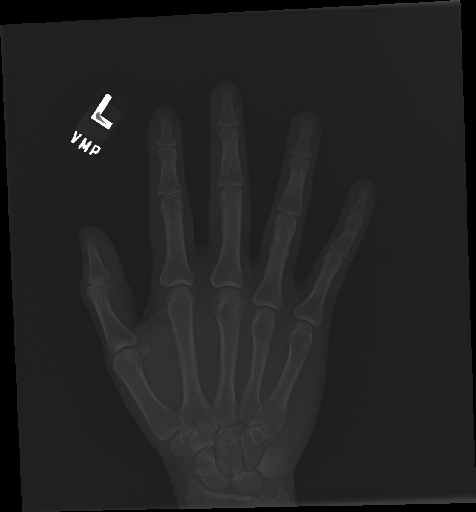
\includegraphics[scale=0.5]{image1.png}
  \caption{Another example X-Ray Image}
  \label{fig:xray2}
  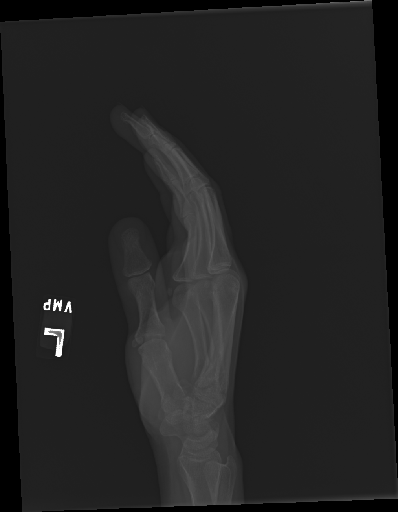
\includegraphics[scale=0.5]{image2.png}
  \caption{A copy of figure 2}
  \label{fig:xray2_copy}
  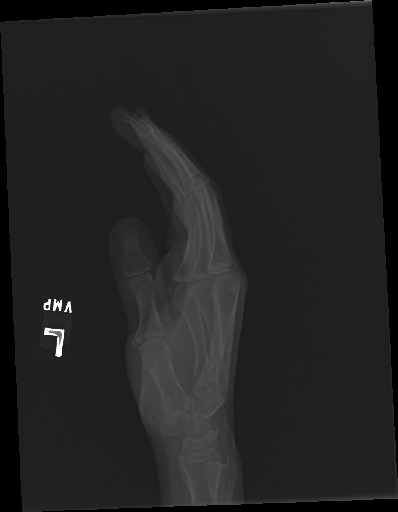
\includegraphics[scale=0.5]{image2_copy.png}
\end{figure}
\clearpage
\noindent

\subsection{Data Breakdowns}
Data breakdowns

% END DATA


% BEGIN MODEL DEVELOPMENT
\newpage
\section{Model Development}

\subsection{Working Environment}
Describe google cloud set-up, GPU, python packages used etc

\subsection{Data Preprocessing}
Describe the preprocessing work done on the data - resize images, normalise values, data augmentation etc 

\subsection{Model}
Describe the final ab-initio model I end up with - structure, loss function, training params/hyperparams etc

\subsection{Predictions}
Discuss getting predictions and aggregating down to study-level predctions

% END MODEL DEVELOPMENT


% BEGIN RESULTS
\newpage
\section{Results}

\subsection{Baseline Performance}
Give the performance of my chosen ab-initio model

\subsection{Image Size}
How do my results vary with size of image? Does increasing image size increase scope for

\subsection{Regularisation}
Perform some regularisation experiments, show results

\subsection{Pre-Trained Models}
How does my model compare vs a selection of pretrained models

% END RESULTS


% BEGIN CONCLUSIONS
\newpage
\section{Conclusions}
Include introspective chapter
Work here not comaparable to clinical setting, e.g. smaller, lower resoution images; radiologist may have a relationship with patient - know medical history, other symptoms etc
What is "abnormal"? - type \& severity of abnormality not known, MURA paper not clear.

% END CONCLUSIONS


% BEGIN ETHICAL
\newpage
\section{Professional and Ethical Issues}
Potential Impact on Radiology - Deep Learning tools used to help triage/prioritise radiologists' work, not replace them; 
Can we trust diagnosis to a computer program? Would you be happy to do so? 
Conversely - medical errors happen a lot (est. cost \$X p.a.; any specifics for radiology?) but DL tools may at least help cut that down.

% END ETHICAL


% BEGIN EXTENSIONS
\newpage
\section{Extensions}
Enquire further about what "abnormal" means
Alternative data e.g. CheXNet, others(?)
Alter NN to accept multiple images simultaneously and so predict based on several views at once (e.g. by weight-sharing, or appening all study images into a single 3D tensor)

% END EXTENSIONS



\clearpage
\bibliographystyle{plain}
\bibliography{bibliography}

\clearpage
\appendix
\section{Pretrained Model Architechtures}
Below we describe the architechtures of the various pre-trained neural network models mentioned in the text.
\subsection{VGG16}
This is the VGG16 model.


\end{document}
